\documentclass[11pt]{report}
\usepackage[a4paper, margin=0.8in]{geometry}
\usepackage[french]{babel}
\usepackage[T1]{fontenc}
\usepackage{amssymb}
\usepackage{pgfplots}
\pgfplotsset{compat=1.15}
\usepackage{mathrsfs}
\usetikzlibrary{arrows}
\usepackage{amsthm}
\usepackage{amsmath}
\usepackage{stmaryrd}
\usepackage[european,straightvoltages,RPvoltages,cute inductors]{circuitikz}
\usetikzlibrary{babel}
\usepackage{listings}
\usepackage{xcolor}
\usepackage{mathtools}
\usepackage{multicol}
\usepackage{xcolor-material}
\usepackage{hyperref}
\usepackage{enumitem}
\usepackage{fancyhdr}
\usepackage{tikz}
\hypersetup{hidelinks}
\usepackage{listings}

\usepackage{siunitx}
\sisetup{
  locale = FR,
  separate-uncertainty,
  inter-unit-product = \cdot
  }
  
\usepackage{pdfpages}
\usepackage{anyfontsize}
\usepackage{setspace}
\addto\captionsfrench{\renewcommand{\chaptername}{Séance}}

\allowdisplaybreaks
\setlength{\parindent}{0pt}

\lstset{
    language=Matlab,
    basicstyle=\small\ttfamily,
    keywordstyle=\color{blue},
    commentstyle=\color{green!60!black},
    stringstyle=\color{purple},
    numbers=left,
    numberstyle=\tiny,
    frame=single,
    breaklines=true
}

\newcommand{\R}{\mathbb{R}}
% Définition d'une couleur sobre pour le titre (gris très foncé)
\definecolor{darkgray}{RGB}{50, 50, 50}

\begin{document}

\begin{titlepage}
    \centering
    
    % --- En-tête ---
    \vspace*{1.5cm}
    {\LARGE \textsc{[Grenoble INP - Esisar]}}\\[1cm]
    {\Large PX222 - AUTO ELEC}\\[2cm]
    
    % --- Titre du document ---
    \textcolor{darkgray}{\rule{\linewidth}{0.8pt}} \\[0.7cm]
    {\Huge \bfseries Carnet de Bord} \\[0.4cm]
    \textcolor{darkgray}{\rule{\linewidth}{0.8pt}} \\[1.5cm]
    
    % --- Sujet ---
    {\Large \textit{Contrôle de courant dans un circuit inductif}} \\[3cm]
    
    % --- Membres du groupe (alignés à gauche) ---
 
    Antton Chevrier \quad Lucas Fernandez \quad Francis Ferguson 
    
    \vfill 
    
    \begin{flushright} \large
        \textbf{Période :} Mars à juin 2026 \\[0.4cm]
        \textit{Dernière mise à jour : \today} 
    \end{flushright}
    
\end{titlepage}

\clearpage

\tableofcontents

\clearpage

\chapter*{Introduction}
L'objectif de ce projet est de réaliser un asservissement de courant dans un circuit inductif, au travers de la bobine étudiée en PX221. Nous utilserons un microcontrôleur STM-32 pour réaliser l'asservissement numérique. 

\begin{figure}[h]
  \begin{center}
    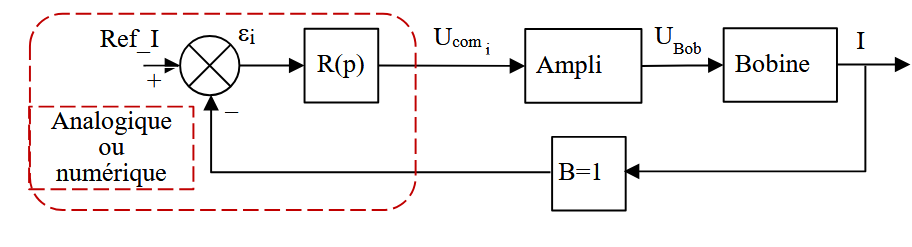
\includegraphics[width=\textwidth]{img/schema_bloc_complet.png}
    \caption{Schéma bloc du montage à réaliser}
  \end{center}
\end{figure}

\chapter{Mercredi 18 mars 2026}

\section{Modélisation des éléments du montage}
Pour commencer, nous avons modélisé les différents éléments du montage à l'aide de leurs fonctions de transfert respectives.

\subsection{Bobine}
Pour l'étude, nous retenons un \textbf{modèle série simple} de la bobine à noyau de fer (BNF). Ce modèle prend en compte l'inductance $L$ représentant l'auto-induction et la résistance série $R$ constituée par l'enroulement en cuivre. 

Nous y ajoutons en série une résistance de puissance $R_{pu} = \qty{12}{\ohm}$ afin de diviser la constante de temps du système par 2. D'après les mesures du semestre précédent (PX221), nous savons que la résistance interne de la bobine est $R = \qty{14}{\ohm}$ et son inductance est $L = \qty{1,2}{\henry}$.

La résistance totale du circuit est donc : $R_{tot} = R + R_{pu} = 14 + 12 = \qty{26}{\ohm}$.

\begin{center}
\begin{circuitikz}
  \draw (0,0) 
      to[vsource, v=$U$] (0,3)
      to [R, l=$R_{pu}$, v<=$U_{R_{pu}}$] (2,3)
      to[R, l=$R$, v<=$U_R$, i=$I$] (5,3)
      to [L, l=$L$, v^=$U_L$] (5,0) --(0,0) ;
\end{circuitikz}
\end{center}

On obtient la fonction de transfert de la charge :
\begin{equation*}
  H_B(p) = \frac{I}{U} = \frac{H_0}{1+\tau p} \quad \text{avec } H_0 = \frac{1}{R_{tot}} = \frac{1}{26} \text{ et } \tau = \frac{L}{R_{tot}} = \frac{1,2}{26} \approx \qty{0,046}{s}
\end{equation*}

\subsection{Amplificateur}
\begin{figure}[h]
  \begin{center}
    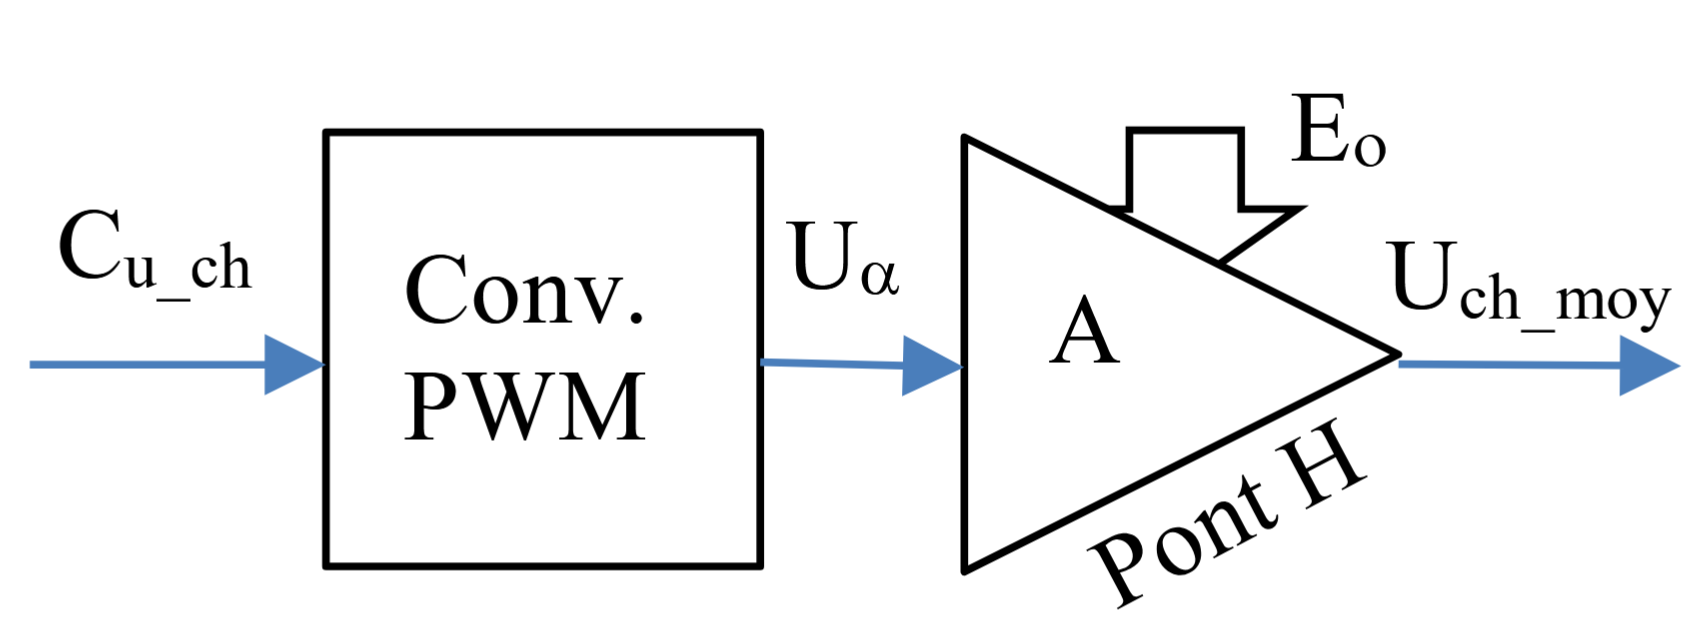
\includegraphics[width=0.3\textwidth]{img/ampli_schema_bloc.png}
    \caption{Schéma bloc fonctionnel de l'amplificateur}
  \end{center}
\end{figure}
L'amplificateur est un dispositif à découpage avec une structure en pont en H. Nous utilisons un \textbf{modèle moyen} pour l'asservissement. En effet, la fréquence de découpage ($f > \qty{20}{kHz}$) est fixée pour être inaudible et est très supérieure à la constante de temps de la charge. Cela permet d'approximer la tension aux bornes de la bobine par sa valeur moyenne $U_{ch_{moy}}$.

D'après le sujet, la tension de sortie est donnée par : $U_{ch_{moy}} = (2 U_{com} - 1)E_0$.
Le gain statique de l'amplificateur est alors défini par la dérivée :
\begin{equation*}
  K_A = \frac{dU_{Bob}}{dU_{com}} = 2E_0
\end{equation*}

\subsection{Capteur de courant}
La mesure du courant s'effectue via la résistance de puissance $R_{pu}$. Le signal traverse un diviseur de tension par 12 pour rester dans la plage de tension de l'électronique, puis un amplificateur d'instrumentation ($U201$). 
Ce montage permet d'obtenir une conversion directe au point de test $TP201$ : $\qty{1}{V} \equiv \qty{1}{A}$.
On en déduit le gain de la chaîne de retour : $B = \qty{1}{V/A}$.

\subsection{Calcul de la boucle ouverte}
La fonction de transfert en boucle ouverte (FTBO) du système complet est :
\begin{align*}
  H_{BO}(p) &= R(p) \cdot K_A \cdot H_B(p) \cdot B \\ 
            &= k \cdot (2E_0) \cdot \frac{\frac{1}{R_{tot}}}{1+\tau p} \cdot 1 \\
            &= \boxed{\frac{\frac{2kE_0}{R_{tot}}}{1+\tau p}}
\end{align*}

\section{Matériel et Sécurité}

\subsection{Liste du matériel prévu}
Pour la mise en œuvre pratique de cet asservissement, nous utiliserons les équipements suivants :
\begin{itemize}
    \item \textbf{Maquette PX222} : Elle servira de base pour le pont en H, les drivers de MOSFET et le conditionnement des signaux.
    \item \textbf{Bobine à Noyau de Fer (BNF)} : Identifiée en PX221, elle constituera notre charge inductive principale ($L \approx \qty{1,2}{H}$).
    \item \textbf{Résistance de puissance (\qty{12}{\ohm})} : Elle sera placée en série pour réduire la constante de temps et servira également au capteur de courant.
    \item \textbf{Microcontrôleur STM32 (Nucleo-F103RB)} : Il sera utilisé pour l'acquisition des signaux (ADC) et la génération de la commande PWM numérique.
    \item \textbf{Appareillage de mesure} : Nous aurons besoin d'un oscilloscope numérique, d'un GBF pour la consigne de courant et de multimètres.
    \item \textbf{Alimentation de puissance} : Une source de tension continue réglable sera utilisée pour alimenter le pont en H (maximum \qty{60}{V}).
\end{itemize}

\subsection{Consignes de sécurité et protocoles}
La manipulation de puissances importantes imposera le respect strict des consignes suivantes :
\begin{itemize}
    \item \textbf{Protection électrique} : Toute tension supérieure à \qty{50}{V} présentant un danger mortel, nous serons donc extremement attentifs lors des essais sous tension.
    \item \textbf{Sondes différentielles} : Pour éviter tout court-circuit via la terre de l'oscilloscope lors des mesures sur le réseau ou le pont flottant, l'usage de sondes différentielles sera obligatoire.
    \item \textbf{Risque thermique} : La résistance de puissance pourra atteindre des températures supérieures à \qty{100}{\degreeCelsius} ; nous éviterons tout contact direct durant et après les essais.
\end{itemize}

\section{Pour la prochaine séance}
Nous devrons avoir terminé les calculs des fonctions de transfert en boucle ouvertes et fermée, ainsi que le calcul du correcteur proportionnel.
\chapter*{Interséance}
Nous avons calculé la fonction de transfert en boucle fermée du système. 

\begin{align*}
  H_{BF}(p) &= \frac{H_{BO}(p)}{1+H_{BO}(p)}\\
            &= \frac{\frac{2kE_0}{R+R_{pu}} \frac{1}{1+\tau p}}{1+\frac{2kE_0}{R+R_{pu}} \frac{1}{1+\tau p}} \\
            &= \frac{K_{BO}}{1+\tau p + K_{BO}} \quad\quad \text{avec } K_{BO} = \frac{2kE_0}{R+R_{pu}}  \\
            &= \frac{\frac{K_{BO}}{1+K_{BO}}}{1 + \frac{\tau p }{1+K_{BO}}}
\end{align*}

On souhaite également une erreur statique de $5\%$. Or
\begin{equation*}
  \varepsilon = \frac{1}{1+K_{BO}} = \frac{1}{1+\frac{2kE_0}{R+R_{pu}}} = 0.05
\end{equation*}
donc \begin{equation*}
  1 + \frac{2kE_0}{R+R_{pu}} = \frac{1}{0.05}
\end{equation*}
d'où \begin{equation*}
  k = \Big(\frac{1}{0.05} -1\Big) \frac{R+R_{pu}}{2E_0}
\end{equation*}
En faisant l'application numérique avec $R+R_{pu} = \qty{26}{\ohm}$ et $E_0 = \qty{60}{V}$, on trouve $k\approx4.1$ 

\chapter{Mardi 31 mars 2026}
Bien que théoriquement, le gain proportionnel de $4$ calculé précédemment fonctionne en théorie, il ne sera pas réalisable en pratique. En effet, le signal de commande $U_{com}$ issu du correcteur doit piloter un convertisseur PWM dont la plage d'entrée est strictement limitée entre \qty{0}{V} et \qty{1}{V}. \\

Pour une consigne unitaire de \qty{1}{A}, un gain $k=4,1$ entraînerait une commande $U_{com} = \qty{4,1}{V}$ dès le début de l'échelon, provoquant une saturation immédiate du rapport cyclique à \qty{100}{\%}. Cette saturation rendrait le système non-linéaire et invaliderait nos modèles de transfert. \\

Nous fixons donc $k=1$ afin de garantir que, même pour une erreur maximale ($\varepsilon = 1$), la commande reste dans la plage linéaire (\qty{1}{V}). Pour compenser l'erreur statique tout en respectant cette contrainte, nous étudions un correcteur Proportionnel-Intégral (PI). \\

Pour le réglage du paramètre d'intégration $\omega_i$, nous utilisons la méthode de \textbf{compensation de pôle}. L'objectif est d'annuler le pôle lent de la bobine ($\tau \approx \qty{0,046}{s}$) en réglant la constante de temps du correcteur telle que $T_i = 1/\omega_i = \tau$. 

Cela donne une valeur théorique de départ :
\begin{equation*}
    \omega_{i} = \frac{1}{\tau} = \frac{R_{tot}}{L} = \frac{26}{1,2} \approx \qty{21,67}{rad/s}
\end{equation*}

Nous utilisons pour cela un script matlab qui nous permet de faire varier $\omega_i$, avec un gain $k=1$ et de visualiser la réponse temporelle du système.

\begin{figure}[h]
  \label{fig:pi}
  \centering
  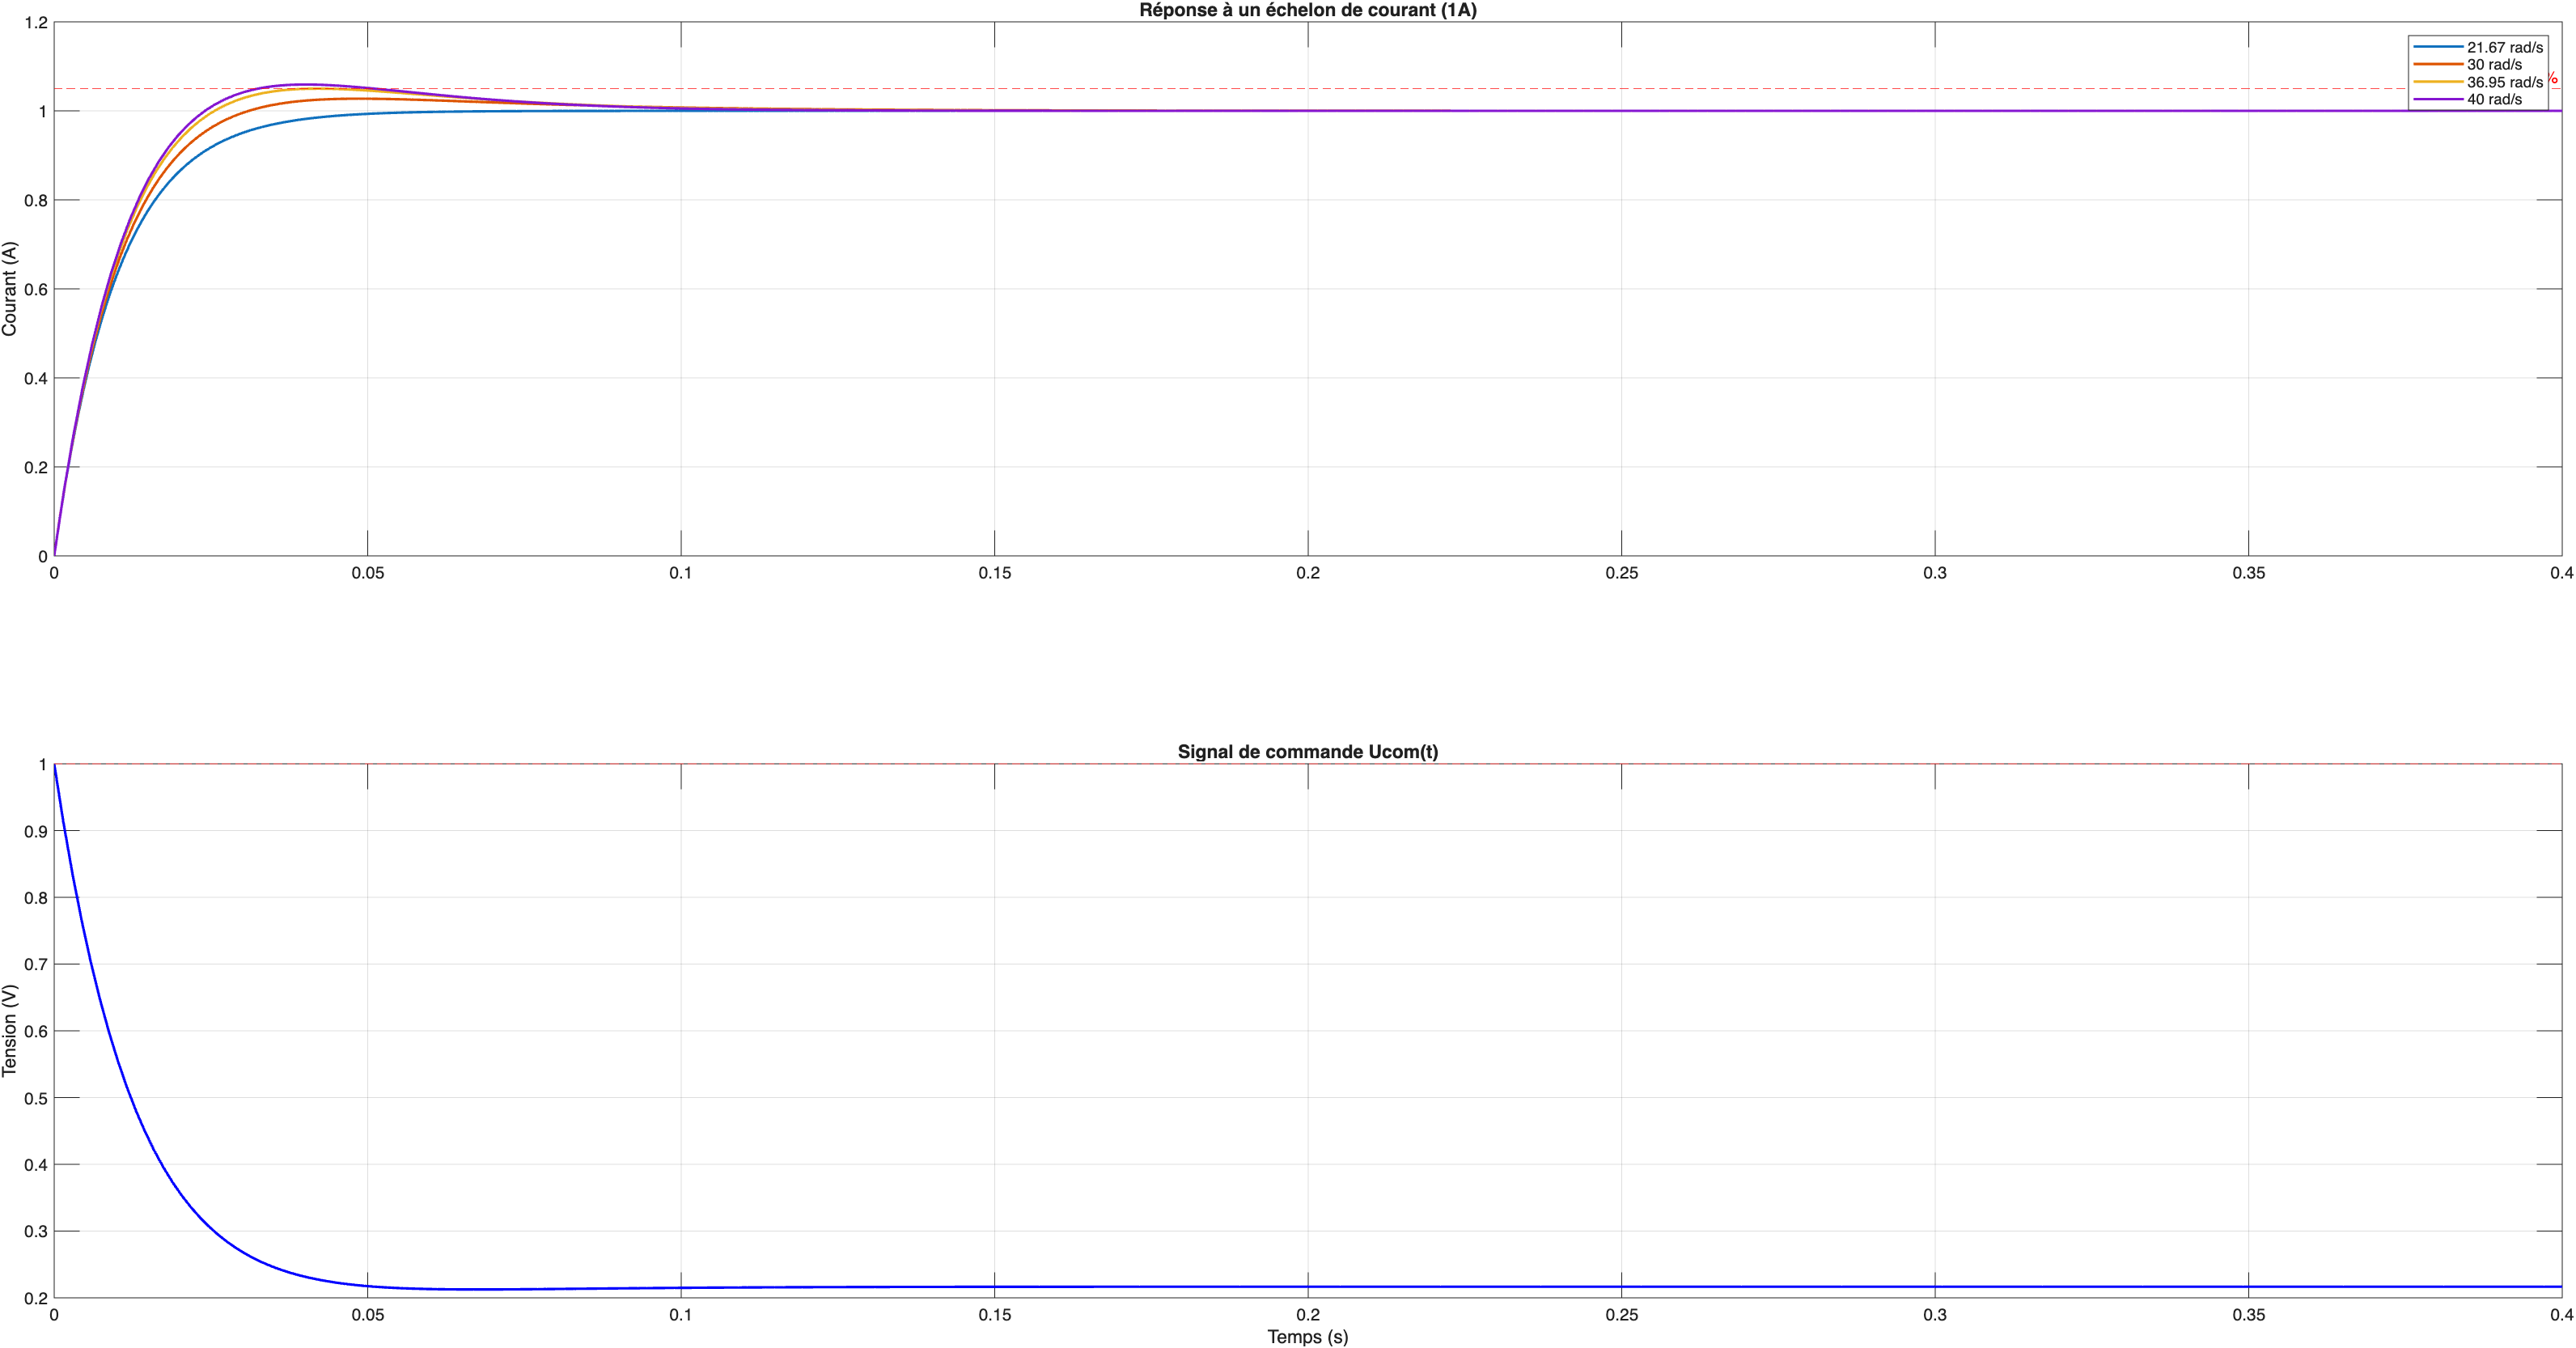
\includegraphics[width=0.8\textwidth]{img/Reponse_PI_et_Commande.png}
  \caption{Réponse temporelle du système pour différentes valeur de $\omega_i$}
\end{figure}

\clearpage

\begin{lstlisting}[language=Matlab, caption={Script Matlab pour trouver le bon paramètre $\omega_i$}, captionpos=b]
% --- Parametres du systeme ---
Rs = 14; 
Rext = 12; 
Rtot = Rs + Rext;
L = 1.2; 
tau = L / Rtot;
E0 = 60; 
Ka = 2 * E0;
B = 1;

s = tf('s');
H_charge = (1/Rtot) / (1 + tau*s);
H = Ka * H_charge * B;

% --- Optimisation du PI ---
k = 1; % Gain fixe pour eviter la saturation
wi_tests = [21.67, 30, 36.95, 40]; % Inclut la compensation de pole

figure('Name', 'Reponse PI et Commande');
for wi = wi_tests
    R = k * (1 + wi/s);
    FTBO = R * H;
    FTBF = feedback(FTBO, 1);
    
    % Analyse des performances
    info = stepinfo(FTBF);
    [y, t] = step(FTBF, 0.4);
    
    subplot(2,1,1); plot(t, y, 'LineWidth', 1.5); hold on;
    fprintf('wi = %.2f | Depassement = %.2f%% | Tr(5%%) = %.3f s\n', ...
            wi, info.Overshoot, info.SettlingTime);
end

% --- Mise en page graphique ---
subplot(2,1,1);
yline(1.05, 'r--', 'Limite 5%'); grid on;
title('Reponse a un echelon de courant (1A)');
ylabel('Courant (A)');
legend(string(wi_tests) + " rad/s");

% Visualisation de la commande pour wi choisi
R_opt = k * (1 + 36.95/s);
Ucom = feedback(R_opt, H); % Transfert Consigne -> Commande
[u, t_u] = step(Ucom, 0.4);
subplot(2,1,2); plot(t_u, u, 'b', 'LineWidth', 1.5); hold on;
yline(1, 'r--', 'Saturation PWM (1V)'); grid on;
title('Signal de commande Ucom(t)');
ylabel('Tension (V)'); xlabel('Temps (s)');
\end{lstlisting}

L'analyse des courbes montre que la valeur $\omega_i = \qty{36,95}{rad/s}$ offre le meilleur compromis. Bien qu'elle soit supérieure à la valeur théorique de compensation, elle permet d'accélérer le système tout en restant sous la limite des \qty{5}{\%} de dépassement.

Les performances simulées sont les suivantes :
\begin{itemize}
    \item \textbf{Dépassement} : \qty{4,92}{\%} (inférieur à la limite de \qty{5}{\%}).
    \item \textbf{Temps de réponse (\qty{5}{\%})} : environ \qty{65}{ms}.
    \item \textbf{Erreur statique} : nulle (grâce à l'action intégrale).
\end{itemize}

\subsection{Analyse du signal de commande}
Le second graphique de la Figure 2.1 présente l'évolution de la tension de commande $U_{com}(t)$. Cette analyse est cruciale pour valider la faisabilité technologique de notre asservissement :

\begin{itemize}
    \item \textbf{Respect de la plage linéaire} : On observe que pour le réglage optimal ($\omega_i = \qty{36,95}{rad/s}$), le signal débute à exactement \qty{1}{V} sans jamais le dépasser. Cela confirme que notre choix $k=1$ permet d'exploiter la dynamique maximale du convertisseur PWM (limité à \qty{1}{V} d'après le sujet) sans jamais saturer le rapport cyclique à \qty{100}{\%}.
    \item \textbf{Effort de commande} : Le pic initial à \qty{1}{V} illustre l'action proportionnelle qui fournit l'énergie nécessaire pour vaincre l'inertie de la charge inductive. La décroissance qui suit montre l'action du terme intégral qui ajuste finement la tension pour stabiliser le courant à \qty{1}{A}, prouvant que le système ne force pas inutilement sur les composants une fois le régime établi.
\end{itemize}

\section{Conclusion de séance}
Pour la prochaine séance, nous devrons nous renseigner sur l’utilisation et la programmation de carte
STM32, notamment sur les différents ports disponibles les différentes façon de brancher les différents
élément du montage à la carte.

\chapter*{Interséance}
\addcontentsline{toc}{chapter}{Interséance}

Suite aux simulations effectuées lors de la séance précédente, nous avons préparé l'implémentation du correcteur PI sur le microcontrôleur STM32 (Nucleo-F103R8) afin de réaliser l'asservissement numérique.

\section*{Stratégie de programmation}
Pour garantir la précision temporelle de l'asservissement, nous avons choisi une programmation par accès direct aux registres. Les choix techniques sont les suivants :
\begin{itemize}
    \item \textbf{PWM (TIM1\_CH1 sur PA8)} : Configuration d'une porteuse à environ \qty{22}{kHz} pour piloter le pont en H de la maquette.
    \item \textbf{Acquisition (ADC1\_IN5 sur PA5)} : Lecture de l'image du courant convertie à \qty{1}{V}/\qty{1}{A} par l'amplificateur d'instrumentation de la carte.
    \item \textbf{Régulation} : Implémentation de la loi de commande avec $k=1$ et $\omega_i = \qty{36,95}{rad/s}$. Une saturation logicielle à \qty{1}{V} est ajoutée pour protéger le système.
\end{itemize}

\section*{Code source concernant les registres et le setup de la carte}
\begin{lstlisting}[language=C, caption={Implémentation du correcteur PI sur STM32F103}, captionpos=b]
#include <stdint.h>

// --- ADRESSES REGISTRES STM32F103 ---
#define RCC_BASE      0x40021000
#define GPIOA_BASE    0x40010800
#define ADC1_BASE     0x40012400
#define TIM1_BASE     0x40012C00

// Horloges
#define RCC_APB2ENR   (*(volatile uint32_t *)(RCC_BASE + 0x18))
#define RCC_CFGR      (*(volatile uint32_t *)(RCC_BASE + 0x04))

// GPIOA
#define GPIOA_CRL     (*(volatile uint32_t *)(GPIOA_BASE + 0x00))
#define GPIOA_CRH     (*(volatile uint32_t *)(GPIOA_BASE + 0x04))

// ADC1 (PA5 est ADC_IN5 sur F103)
#define ADC1_SR       (*(volatile uint32_t *)(ADC1_BASE + 0x00))
#define ADC1_CR2      (*(volatile uint32_t *)(ADC1_BASE + 0x08))
#define ADC1_SQR3     (*(volatile uint32_t *)(ADC1_BASE + 0x34))
#define ADC1_DR       (*(volatile uint32_t *)(ADC1_BASE + 0x4C))

// TIM1 (PWM sur PA8)
#define TIM1_CR1      (*(volatile uint32_t *)(TIM1_BASE + 0x00))
#define TIM1_PSC      (*(volatile uint32_t *)(TIM1_BASE + 0x28))
#define TIM1_ARR      (*(volatile uint32_t *)(TIM1_BASE + 0x2C))
#define TIM1_CCR1     (*(volatile uint32_t *)(TIM1_BASE + 0x34))
#define TIM1_CCMR1    (*(volatile uint32_t *)(TIM1_BASE + 0x18))
#define TIM1_CCER     (*(volatile uint32_t *)(TIM1_BASE + 0x20))
#define TIM1_BDTR     (*(volatile uint32_t *)(TIM1_BASE + 0x44))

void setup(void) {
    // 1. Activer horloges : GPIOA, ADC1, TIM1 et AFIO
    RCC_APB2ENR |= (1 << 0) | (1 << 2) | (1 << 9) | (1 << 11);

    // 2. Configurer PA8 en "Alternate Function Push-Pull" (PWM TIM1_CH1)
    GPIOA_CRH &= ~(0xF << 0);
    GPIOA_CRH |= (0xB << 0); // Speed 50MHz, AF Push-Pull

    // 3. Configurer PA5 en mode Analogique (Entree mesure courant)
    GPIOA_CRL &= ~(0xF << 20);

    // 4. Configurer TIM1 pour PWM a 22kHz
    TIM1_PSC    = 0;              // Pas de diviseur
    TIM1_ARR    = 3272;           // 72MHz / 22kHz environ = 3272
    TIM1_CCMR1 |= (0x6 << 4);  // Mode PWM 1 sur CH1
    TIM1_CCER  |= (1 << 0);     // Activer sortie CH1
    TIM1_BDTR  |= (1 << 15);    // Main Output Enable (MOE) - Specifique TIM1
    TIM1_CR1   |= (1 << 0);      // Lancer Timer

    // 5. Configurer ADC1
    ADC1_SQR3 = 5;             // Selectionner canal 5 (PA5)
    ADC1_CR2 |= (1 << 0);      // Allumer ADC
}

uint32_t read_ADC(void) {
    ADC1_CR2 |= (1 << 22);     // Lancer conversion
    while (!(ADC1_SR & (1 << 1))); // Attendre fin
    return ADC1_DR;
}

void delay_ms(uint32_t ms) {
    for (uint32_t i = 0; i < ms * 8000; i++) __asm__("nop");
}



\end{lstlisting}
\section*{Code source concernant les calculs du correcteur PI et de la commande}
\begin{lstlisting}[language=C, caption={Implémentation du correcteur PI sur STM32F103}, captionpos=b]
// --- PARAMETRES DU CORRECTEUR PI ---
const float Kp = 1.0f;           // Gain proportionnel
const float Wi = 36.95f;        // Parametre d'integration
const float Ts = 0.001f;        // Periode d'echantillonnage (1ms)
float integrale = 0.0f;
float consigne = 1.0f;          // 1V <=> 1A

    while (1) {
        // --- 1. ACQUISITION ---
        uint32_t val_adc = read_ADC();
        // Conversion ADC (12 bits) en Volts : val * 3.3 / 4095
        float courant_mesure = (float)val_adc * (3.3f / 4095.0f);

        // --- 2. CALCUL DU PI ---
        float erreur = consigne - courant_mesure;
        integrale += erreur * Ts;

        // Commande = Kp * (erreur + Wi * integrale)
        float commande = Kp * (erreur + Wi * integrale);

        // --- 3. SATURATION ET PROTECTION ---
        // On bride la commande entre 0 et 1V pour rester en zone lineaire
        if (commande > 1.0f) commande = 1.0f;
        if (commande < 0.0f) commande = 0.0f;

        // --- 4. ACTION (PWM) ---
        // Le rapport cyclique est proportionnel a la commande (0V=0, 1V=100%)
        // On ramene la commande 0-1V vers l'ARR du Timer (3272)
        TIM1_CCR1 = (uint32_t)(commande * 3272.0f);

        delay_ms(1); // Echantillonnage a 1kHz
    }

\end{lstlisting}
\end{document}